\section{Performance comparison}

This section is the core of this work. In here, all the metrics developed and
used for the carrying out the performance comparison are explained in detail
together with the justification on why they were selected.

All the simulations were performed considering a non-dimensional radius of
$\rho=\norm{\vec{r_2}}/\norm{\vec{r_1}}=2$ and unitary gravitational parameter
$\mu=1$ [L3, T2], where L3 and T2 stand for units of cubic length and squared
time respectively. The problem was solved for a variety of transfer angles
$\Delta \theta$ between $0$ and $2\pi$ and non-dimensional transfer times $\tau$
within the same range of values. For this last parameter, equation
\ref{eq:non_dimensional_tof}:

\begin{equation}
  \tau =  \Delta t \cdot \sqrt{\frac{8\mu}{s^3}}
  \label{eq:non_dimensional_tof}
\end{equation}

By making use of previous equation, each revolution solution lies within an
interval which is a multiple of $2\pi$. For example, the direct transfer problem
will have the solution within the $[0, 2\pi)$ interval, while for the
multiple-revolution scenario, the interval changes to $[2\pi M, 2\pi(M+1))$.

As it has been introduced in several sections, this work only covers the direct
arc transfer, meaning that the multi-revolution scenario is not studied. All
orbits were assumed to be \textit{prograde} and no distinction between
\textit{low} or \textit{short} paths was required as multiple solutions only
appear in the multi-revolution problem. The absolute tolerance was set to $1e-5$
and the relative one to $1e-7$.

The three metrics used in this report are:

\begin{itemize}
  \item \textbf{Number of iterations}: this metric provides information about
        the convergence of the numerical method but also about the initial
        guess. Because the initial guess outputs an estimate solution, the
        accurate this routine is, the lower the amount of iterations required
        by the numerical method.
  \item \textbf{Time per iteration}: which measures the mean time required for
        computing a new approximate value of the free-parameter. This metric
        reveals more information about the time consumed by the numerical
        method.
  \item \textbf{Total computation time}: which computes the total time required
        during the iteration workload. Measuring the whole computation time of
        a solver would have an impact in the results due to the implementation
        of the algorithm.
\end{itemize}

\subsection{Number of iterations}

The first metric used for the performance comparison is the amount of iterations
it takes for a solver to achieve the solution for a given combination of $\Delta
  \theta$ and $\Delta \tau$. Black regions show for which points the algorithm did
not converged, either because of the accuracy or the method itself.

Gauss' solver, in figure \ref{fig:iter_gauss}, reveals that the method is only
valid for lower transfer angle and non-dimensional times. This situation was
already known and claimed by several authors in literature. On the other hand,
the improved version of the method by Battin, see \ref{fig:iter_battin}
converges for any case and the imposed absolute tolerance. These last method is
seen to be more robust and accurate than Gauss one.

The solver devised by Gooding shows an stable behavior for most of the solution
space, only requiring between two and three iterations, \ref{fig:iter_gooding}.
This is due to the strong initial guess together with the usage of Halley's
method.

Regarding Avanzini's solver, this algorithm exhibits a lower number of
iterations for transfer angles of the same value of the non-dimensional time of
flight. For corner cases, see \ref{fig:iter_avanzini}, the iterations increase up
to eight or nine. Even with that, the solution is found in all of the cases,
meaning that the algorithm converged without any problem.

Arora's algorithm, in figure \ref{fig:iter_arora}, is seen to be the most stable
one, requiring a mean of only two iterations. This algorithm holds the most
complex initial guess procedure of all the solvers presented in this work, which
together with Halley's method explains the lower amount of iterations.
Convergence is ensured with this solver.

Vallado's solver also converged to the majority of the cases, except for those
ones with low time of flight. However, due to the bisection method employed, the
number of iterations increases dramatically. This can be seen in figure
\ref{fig:iter_vallado}.

Finally, Izzo's solver in figure \ref{fig:iter_izzo} is also seen to be stable
and robust for the majority of the cases. Only values around $\tau=\pi/2$
require more than two iterations, no matter the transfer angle.


% --- START: NUMBER OF ITERATIONS FIGURES ---
\begin{figure}[H]
  \begin{minipage}{0.48\textwidth}
    \centering
    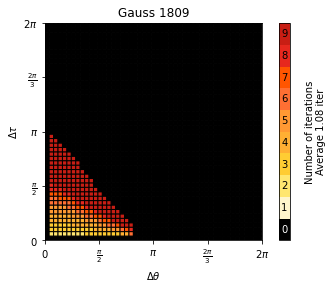
\includegraphics[width=1.05\linewidth]{static/iter/iter_gauss_1809.png}
    \caption{Gauss' iterations.}\label{fig:iter_gauss}
  \end{minipage}\hfill
  \begin{minipage}{0.48\textwidth}
    \centering
    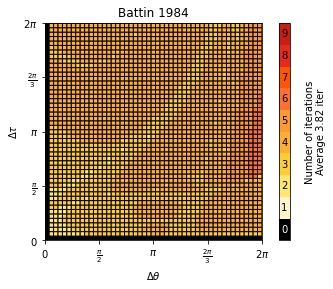
\includegraphics[width=1.05\linewidth]{static/iter/iter_battin_1984.png}
    \caption{Battin's iterations.}\label{fig:iter_battin}
  \end{minipage}
\end{figure}

\begin{figure}[H]
  \begin{minipage}{0.48\textwidth}
    \centering
    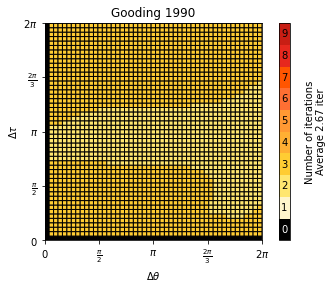
\includegraphics[width=1.05\linewidth]{static/iter/iter_gooding_1990.png}
    \caption{Gooding' iterations.}\label{fig:iter_gooding}
  \end{minipage}\hfill
  \begin{minipage}{0.48\textwidth}
    \centering
    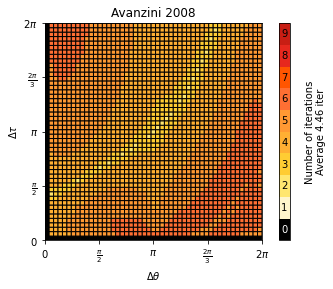
\includegraphics[width=1.05\linewidth]{static/iter/iter_avanzini_2008.png}
    \caption{Avanzini's iterations.}\label{fig:iter_avanzini}
  \end{minipage}
\end{figure}

\begin{figure}[H]
  \begin{minipage}{0.48\textwidth}
    \centering
    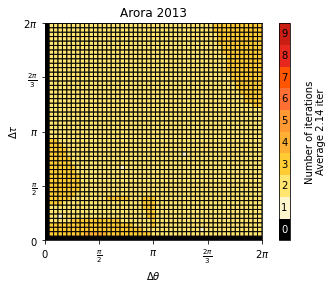
\includegraphics[width=1.05\linewidth]{static/iter/iter_arora_2013.png}
    \caption{Arora' iterations.}\label{fig:iter_arora}
  \end{minipage}\hfill
  \begin{minipage}{0.48\textwidth}
    \centering
    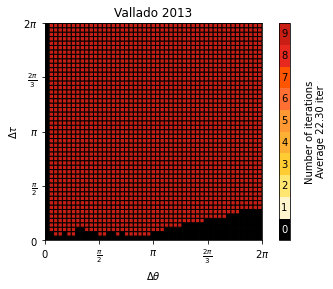
\includegraphics[width=1.05\linewidth]{static/iter/iter_vallado_2013.png}
    \caption{Vallado's iterations.}\label{fig:iter_vallado}
  \end{minipage}
\end{figure}

\begin{figure}[H]
  \begin{minipage}{0.48\textwidth}
    \centering
    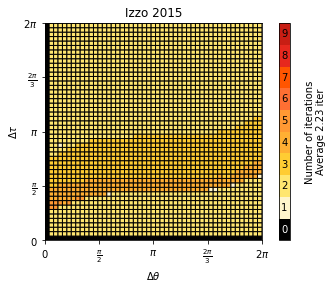
\includegraphics[width=1.05\linewidth]{static/iter/iter_izzo_2015.png}
    \caption{Izzo's iterations.}\label{fig:iter_izzo}
  \end{minipage}\hfill
  \begin{minipage}{0.48\textwidth}
    \centering
    
\includegraphics[width=1.05\linewidth]{static/void_figure.png}
  \end{minipage}
\end{figure}
% --- END: NUMBER OF ITERATIONS FIGURES ---

\subsection{Time per iteration}

A solver may require a huge number of may require a huge number of iterations.
However, if each one of those only needs a minimum amount of time, the overall
computation might be a high performance one. In this subsection, the time per
iteration of each one of the solvers is presented.

It is important to state that the time required for a computer to solve a
particular problem might slightly vary due to internal processes which have
nothing to do with the computation process itself. Therefore, the problem was
solved multiple times and the mean iteration time. Let us now present the
results.

For the case of Gauss' solver, the time consumed per iteration is stable as
depicted by figure \ref{fig:tpi_gauss}. On the other hand, Battin's solver in
figure \ref{fig:tpi_battin} shows a reduction in the time per iteration for low
values of the canonical transfer time. However, this last solver requires more
time than Gauss one due to the complexity of the method used. Nevertheless, it
converges for all cases, which is a major advantage over speed as a solution is
found.

Gooding's solver in \ref{fig:tpi_gooding} only shows an critical region near
non-dimensional times of $\tau=\pi/2$. For the rest of the cases, the time per
iteration is quite low and stable. Halley's method is proof to be fast when
carrying out the iteration workload.

The algorithm requiring the greatest amount of time per iteration is Avanzini's
one, see figure \ref{fig:tpi_avanzini}. This solver requires more time for the
regions in which it employed less iterations.

Arora's solver, on the other hand, shows an overall time per iteration slightly
greater than Gooding's one. Even with that, the solver only experiences an
increase in the computation of the time per iteration for values below of
$\tau=\pi/2$. The diagram for this solver is shown in figure
\ref{fig:tpi_arora}.

Vallado's solver, in figure \ref{fig:tpi_vallado} shows now a closer behavior
to the rest of the solvers when discussing the time per iteration. This is due
to the bisection method employed by the solver, as this root solver is fast from
the time per iteration point of view but requires a huge amount of iterations
for achieving the desired absolute tolerance.

The last of the solvers, Izzo's one in figure \ref{fig:tpi_izzo} is not as
stable as Gooding's or Arora's algorithms, but also shows a great stability and
performance for the iteration workload. As similar to Arora's, this solver
experiences and increase in the time per iteration for values of $\tau=\pi/2$.


% --- START: NUMBER OF TIME PER ITERATION FIGURES ---
\begin{figure}[H]
  \begin{minipage}{0.48\textwidth}
    \centering
    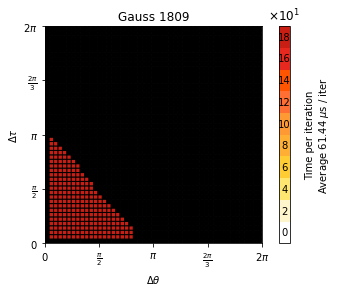
\includegraphics[width=1.05\linewidth]{static/tpi/tpi_gauss_1809.png}
    \caption{Gauss' time per iter.}\label{fig:tpi_gauss}
  \end{minipage}\hfill
  \begin{minipage}{0.48\textwidth}
    \centering
    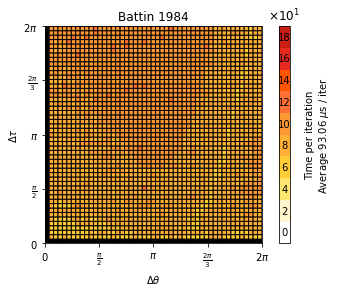
\includegraphics[width=1.05\linewidth]{static/tpi/tpi_battin_1984.png}
    \caption{Battin's time per iter.}\label{fig:tpi_battin}
  \end{minipage}
\end{figure}

\begin{figure}[H]
  \begin{minipage}{0.48\textwidth}
    \centering
    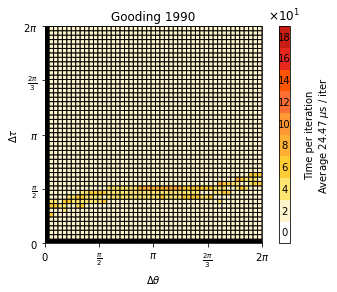
\includegraphics[width=1.05\linewidth]{static/tpi/tpi_gooding_1990.png}
    \caption{Gooding' time per iter.}\label{fig:tpi_gooding}
  \end{minipage}\hfill
  \begin{minipage}{0.48\textwidth}
    \centering
    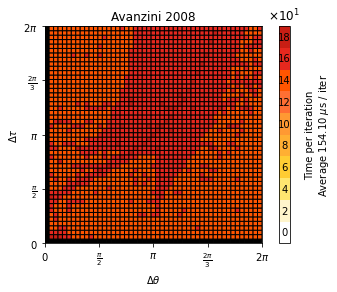
\includegraphics[width=1.05\linewidth]{static/tpi/tpi_avanzini_2008.png}
    \caption{Avanzini's time per iter.}\label{fig:tpi_avanzini}
  \end{minipage}
\end{figure}

\begin{figure}[H]
  \begin{minipage}{0.48\textwidth}
    \centering
    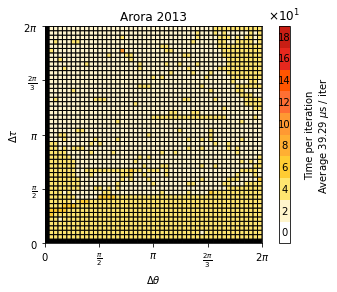
\includegraphics[width=1.05\linewidth]{static/tpi/tpi_arora_2013.png}
    \caption{Arora' time per iter.}\label{fig:tpi_arora}
  \end{minipage}\hfill
  \begin{minipage}{0.48\textwidth}
    \centering
    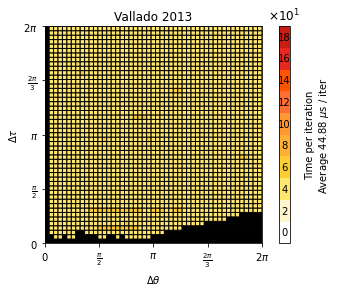
\includegraphics[width=1.05\linewidth]{static/tpi/tpi_vallado_2013.png}
    \caption{Vallado's time per iter.}\label{fig:tpi_vallado}
  \end{minipage}
\end{figure}

\begin{figure}[H]
  \begin{minipage}{0.48\textwidth}
    \centering
    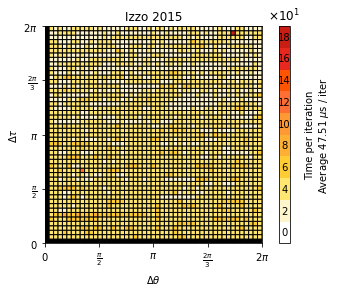
\includegraphics[width=1.05\linewidth]{static/tpi/tpi_izzo_2015.png}
    \caption{Izzo's time per iter.}\label{fig:tpi_izzo}
  \end{minipage}\hfill
  \begin{minipage}{0.48\textwidth}
    \centering
    
\includegraphics[width=1.05\linewidth]{static/void_figure.png}
  \end{minipage}
\end{figure}
% --- END: TIME PER ITERATION FIGURES ---






\subsection{Total computation time}
